% Original abstract learning landscape; all shapes are editable TikZ paths.
% Copyright (C) 2026 Xiao Fan <xiaofan140@gmail.com>
% SPDX-License-Identifier: GPL-3.0-or-later
\documentclass[tikz,border=0pt]{standalone}
\definecolor{brand}{HTML}{000000}
\begin{document}
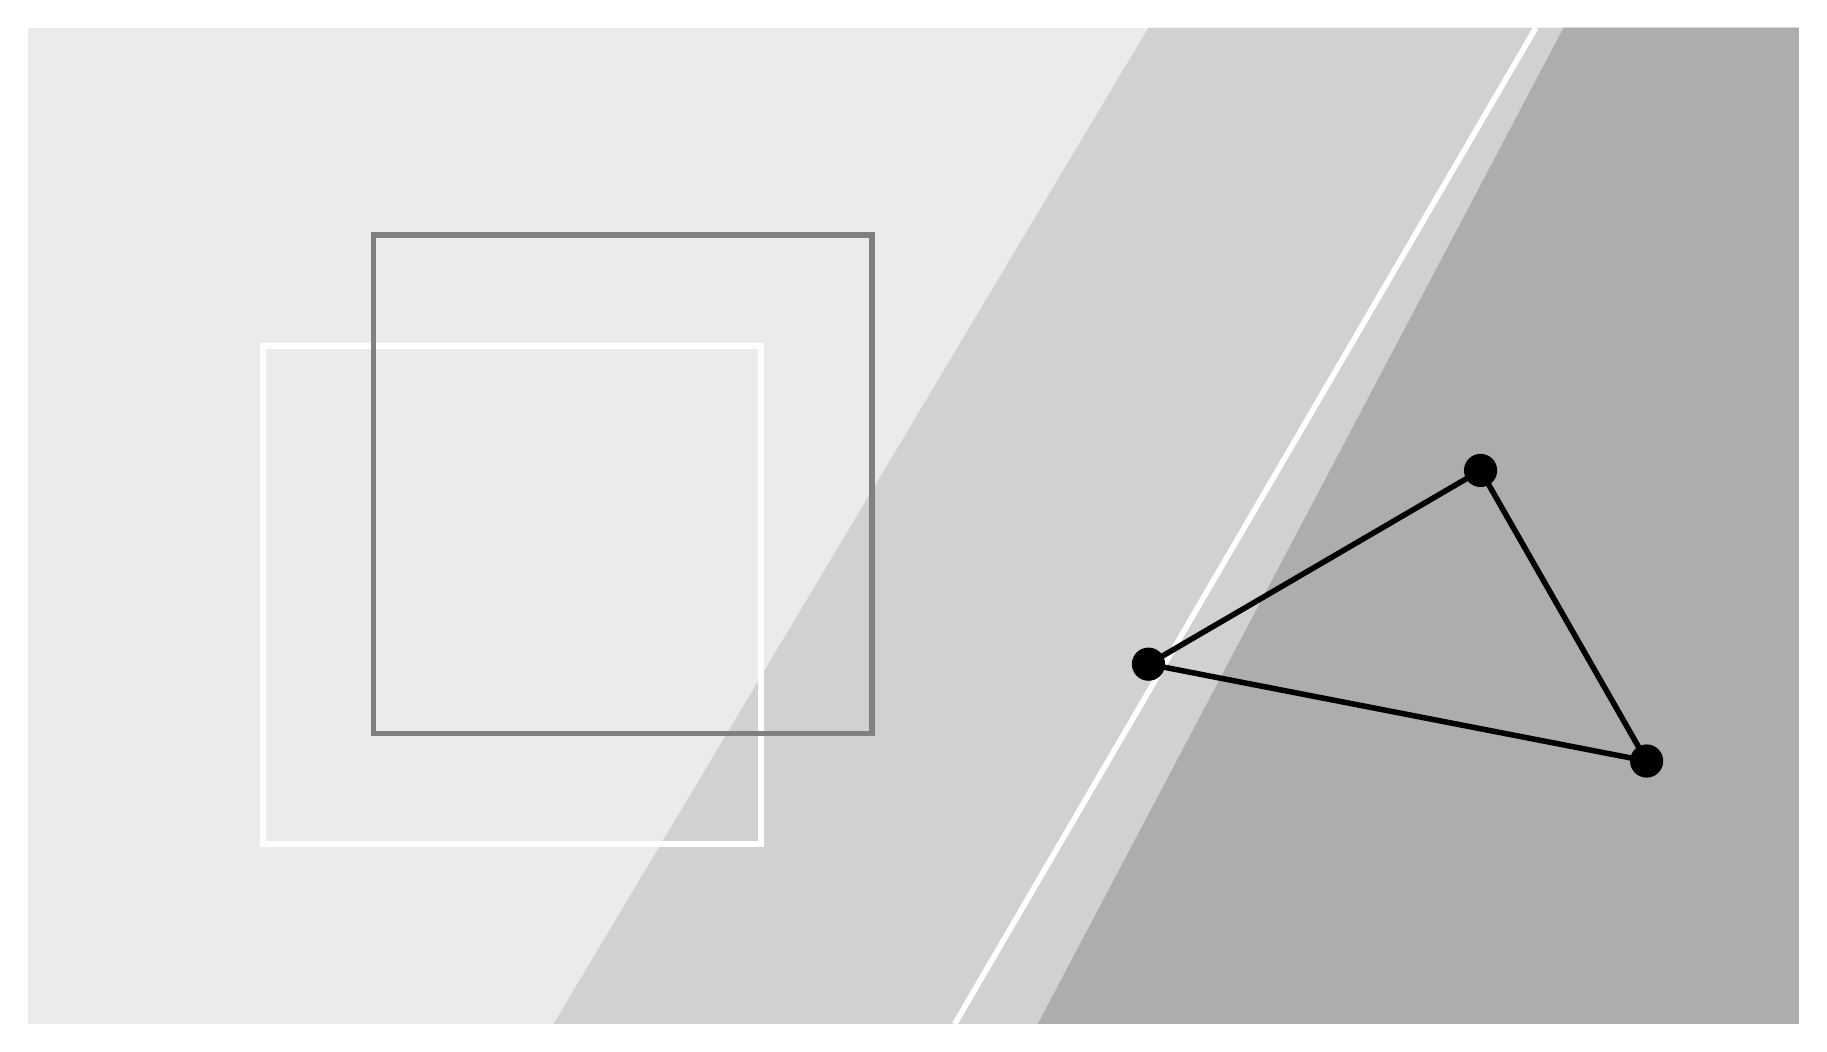
\begin{tikzpicture}[x=1pt,y=1pt]
  \clip (0,0) rectangle (640,360);
  \fill[brand!8] (0,0) rectangle (640,360);
  \fill[brand!18] (190,0) -- (405,360) -- (640,360) -- (640,0) -- cycle;
  \fill[brand!32] (365,0) -- (555,360) -- (640,360) -- (640,0) -- cycle;
  \draw[white,line width=2] (335,0) -- (545,360);
  \draw[white,line width=2] (85,65) -- (265,65) -- (265,245) -- (85,245) -- cycle;
  \draw[brand!50,line width=2] (125,105) -- (305,105) -- (305,285) -- (125,285) -- cycle;
  \fill[brand] (405,130) circle (6);
  \fill[brand] (525,200) circle (6);
  \fill[brand] (585,95) circle (6);
  \draw[brand,line width=2] (405,130) -- (525,200) -- (585,95) -- cycle;
\end{tikzpicture}
\end{document}
